%-------------------------------------------------------------------------
\documentclass[number,preprint,review,12pt]{elsarticle}

\usepackage{hyperref}				% enlaces en el pdf
\hypersetup{colorlinks=true}	    % colores en vez de cajas en los enlaces
\usepackage{times}              	% la letra
\usepackage{graphicx}           	% para manejar imagenes
\usepackage{tabularx}		   		% para ajustar el ancho de las columnas
\usepackage{algorithm}				% Para el seudocódigo
\usepackage{setspace}				% Para el seudocódigo
\usepackage{amsmath}				% Para el seudocódigo
\usepackage[noend]{algpseudocode}	% Para el seudocódigo
\usepackage{multicol}				% Para el seudocódigo

\newtheorem{proposition}{Proposition}
\newtheorem{definition}{Definition}
\newtheorem{corollary}{Corollary}

% Change algorithm input/output
\renewcommand{\algorithmicrequire}{\textbf{Input:}}
\renewcommand{\algorithmicensure}{\textbf{Output:}}

\newcolumntype{L}[1]{>{\raggedright\let\newline\\\arraybackslash\hspace{0pt}}m{#1}}
\newcolumntype{C}[1]{>{\centering\let\newline\\\arraybackslash\hspace{0pt}}m{#1}}
\newcolumntype{R}[1]{>{\raggedleft\let\newline\\\arraybackslash\hspace{0pt}}m{#1}}

% Hyphenation
\hyphenation{SBDM}
\hyphenation{SBDMs}

\begin{document}

	\title{A New Algorithm for Reduct Computation based on Gap Elimination and Attribute Contribution}
	
	\author[inaoe,uc]{Vlad\'{\i}mir~Rodr\'{\i}guez-Diez\corref{cor1}}
	\ead{vladimir.rodriguez@ccc.inaoep.mx}
	\author[inaoe]{Jos\'{e}~Fco.~Mart\'{\i}nez-Trinidad}
	\author[inaoe]{Jes\'{u}s~A.~Carrasco-Ochoa}	
	\author[inaoe]{Manuel S.~Lazo-Cort\'{e}s}
	\address[inaoe]{Computer Science Department\\
					Instituto Nacional de Astrof\'{\i}sica, \'{O}ptica y Electr\'{o}nica\\
					Luis Enrique Erro \# 1, Santa Mar\'{\i}a Tonantzintla, Puebla, 72840, M\'{e}xico} 
	\address[uc]{Electrical Engineering Department\\
				 Universidad de Camag\"{u}ey\\
				 Circv. Nte. km 5$\frac{1}{2}$, Camag\"{u}ey, Cuba}
	
	\begin{abstract}
		Attribute reduction is a key aspect of Rough Set Theory.  Finding the complete set of reducts is important for solving problems such as the assessment of attribute relevance, multi--objective cost--sensitive attribute reduction and dynamic reduct computation. The main limitation in the application of Rough Set methods is that finding all reducts of an information system has exponential complexity regarding the number of attributes. Several algorithms have been reported to reduce the cost of reduct computation. Unfortunately, most of these algorithms relay on high cost operations for candidate evaluation. Therefore, in this paper, we propose a new algorithm for computing all reducts of an information system, based on the pruning properties of \textit{gap  elimination} and \textit{attribute contribution}, that uses simpler operations for candidate evaluation in order to reduce the algorithm runtime. Finally, the proposed algorithm is evaluated and compared against other state of the art algorithms, over synthetic and real information systems.
	\end{abstract}
	
	\begin{keyword}
		Rough Sets\sep Reduct Computation\sep Typical Testor.
	\end{keyword}

	\maketitle

%-------------------------------------------------------------------------------
% your earth-shattering contribution

\section{Introduction}
  Rough Set Theory (RST), proposed by Z. Pawlak in 1981 \citep{Pawlak81,Pawlak81-2,Pawlak82,Pawlak91}, 
  is a relatively new mathematical theory to deal with imperfect knowledge, in particular with vague 
  concepts. Into RST, information systems are tables of objects (rows) described by a set of attributes (columns). 
  When data is collected or recorded, every single aspect (attribute) of the objects under study is
  %TODO indivisible considered
  considered to have a complete representation and to ensure that no potentially useful information is lost. As a result, information systems are usually characterized by a large number of attributes, which degrades the performance of machine learning tools \citep{Parthalain08}. One of the main concepts in RST is the notion of reduct, which is a minimal subset of attributes preserving the discernibility capacity of the whole set of attributes \citep{Pawlak91}. However, the main restriction in practical applications of RST is that computing all reducts of an information system is NP--hard \citep{Skowron92}. 
   
   RST reducts have been related to Typical Testors (TT) from the logical combinatorial approach to pattern recognition \citep{Chikalov2013}. Testor Theory was originally created by Cheguis and Yablonskii \cite{Cheguis55} as a tool for analysis of problems connected with control and diagnosis of faults in circuits.  However, Testor Theory has been extended in order to be used for feature selection as shown in \citep{Dmitriev1966,Martinez01,Ruiz08}.

  The complete set of reducts of an information system is needed for solving some practical problems and real--world applications. In \cite{Xu2013} a multi-objective cost-sensitive attribute reduction was developed. First, they compute all reducts of an information system. Then, they separately calculate the cost, in terms of time and money, of every reduct. Finally, the worst reducts are dismissed, leaving a Pareto optimal solution set. From this smaller set of reducts, a user selects an attribute subset. On the other hand, in \cite{Mukamakuza2014} three new algorithms for dynamic reduct computation were developed. The first step in the three algorithms is finding all reducts. Then, the complete set of reducts is filtered in order to obtain an optimum subset, from which dynamic reducts are computed. They showed that this procedure improves the performance of dynamic reduct computation algorithms. From Testor Theory \cite{Torres2014}, the informational weight, computed through the whole set of typical testors (reducts), was used to identify risk factors on transfusion related to acute lung injury; and to establish an assessment for each attribute.  
  %In \citep{Torres2014}, the informational weight of an attribute is computed as the percentage of times the attribute appears in the whole set of typical testors. This computation is not possible without the complete set of typical testors.
  
  Recently, the relation between reduct computation and the minimum vertex cover problem in graph theory was exposed \cite{chen2015}. Given that both of these problems can be translated into the calculation of prime implicants of a Boolean function, they applied algorithms designed for reduct computation in the solution of the minimum vertex cover problem. This unification opens a new spectrum of real-world applications for fast reduct computation algorithms. They stood that the vertex cover problem has been used in applications such as crew scheduling~\citep{Sherali1984}, VLSI design \citep{Bhattacharyya2000}, nurse rostering \citep{Caprara1998} and industrial machine assignments~\citep{Woodyatt1993}. The connection with the problem of computing the prime implicants of a Boolean function makes fast algorithms for computing all reducts relevant in other applications. For instance, in \cite{Li2015} a new technique for mining frequent patterns from the minimal disjunctive normal form was presented.

  In this work, we propose a new algorithm, GCreduct, for computing all reducts based on the pruning properties of Gap elimination and attribute Contribution. 
  %Additionally, we show the advantages of fast binary cumulative operations used in \citep{Sanchez10,Lias13} over other approaches from rough set theory \citep{WangP07,Jensen14}. 
  In relation to fast--BR \citep{Lias13}, which is one of the latest and fastest reported algorithms; our proposed algorithm evaluates more candidates in most cases, but the evaluation cost is lower. Finally, we show that our algorithm performs faster than all other recent reported alternatives in a specific kind of information systems. 
  
  The rest of this paper is structured as follows. Section~\ref{basicConcepts}  introduces some basic concepts. In Section~\ref{relatedWork}, we discuss the related work on reduct and typical testor computation.  In Section~\ref{GCreduct}, we introduce the GCreduct algorithm for computing all reducts of an information system. An evaluation of the proposed algorithm and a discussion of the experimental results are presented in section~\ref{evaluation}. Finally, section~\ref{conclusions} shows our conclusions and some directions for future work.
   
\section{Basic Concepts}\label{basicConcepts}
  RST is based on the assumption that every object in the universe of discourse is described, through a set of attributes, by some information associated to it. This information constitutes the basis for the classification of unseen objects. RST motto is \textit{Let the data speak for themselves} \citep{Tiwari14}.

  From the RST point of view, two objects are indistinguishable (indiscernible) if they have the same value for each attribute in their description. Indiscernibility relations arising in this way constitute the mathematical foundations of RST. Some basic concepts of RST are presented bellow.
  
\subsection{Information System}
  The basic representation of data in RST is an \emph{Information System} (IS). An IS is a table with rows
  representing objects while columns specify attributes or features. Formally, an IS is defined as a pair
  $IS=(U,A)$ where $U$ is a finite non-empty set of objects $U=\lbrace x_1,x_2,...,x_n\rbrace$ and $A$ is a 
  finite non-empty set
  of attributes (features, variables). Every attribute in $A$ is a map: $a: U \rightarrow V_a$. The set $V_a$ is
  called the \textit{value set} of $a$. Attributes in $A$ are further divided into condition attributes $C$ and 
  decision attributes $D$ such that $A=C \cup D$ and $C \cap D =\emptyset$. 
  Table~\ref{tab_IS} shows an example of an IS.
  
 \begin{table}[htb]
		\caption{Example of an Information System, where $c_0-c_6$ are condition attributes and $d$ is a decision attribute.} \label{tab_IS}
		\centering
 	\begin{tabular}{c||c|c|c|c|c|c|c||c}
 			  & $c_0$ & $c_1$ & $c_2$ &  $c_3$ & $c_4$ & $c_5$ &  $c_6$ & $d$ \\
 		\hline \hline
		$x_1$ &   blue  & 0 & medium & 3 & 20 & $<1$  & 1 & bad   \\
		$x_2$ &   red   & 1 & medium & 2 & 20 & $<1$  & 1 & bad   \\
		$x_3$ &   red   & 0 & medium & 3 & 20 & $<1$  & 1 & good   \\
		$x_4$ &   red   & 0 & medium & 3 & 20 & $<1$  & 0 & bad   \\
		$x_5$ &   red   & 0 & long   & 3 & 12 & $<1$  & 1 & bad   \\
		$x_6$ &   green & 0 & short  & 3 & 20 & $=1$  & 1 & good   \\
		$x_7$ &   red   & 0 & medium & 3 & 20 & $=1$  & 1 & bad   \\
		$x_8$ &   red   & 0 & short  & 3 & 20 & $>1$  & 1 & bad   \\
 	\end{tabular}             
 \end{table}
 
  \textit{Decision attributes} determine the class an object belongs to. In the IS of table~\ref{tab_IS}, $d$ is the decision attribute; this is a two-class system. \textit{Condition attributes} do not absolutely determine the class but help to decide which class an object belongs to. In supervised classification, condition attributes are the only information available for classifying new objects; while, decision attributes are only available for objects in the training set. An IS with decision and condition attributes is called a decision system.
  
\subsection{Positive Region}\label{subsect_Pos}
  Decision attributes $D$ induce a partition of the universe $U$ into equivalence classes (\textit{decision classes}). Since we will be trying to associate a decision class to an object based on the attributes belonging to $B \subseteq C$, we are interested in those $B-classes$ (classes induced by $B$) which correspond to the decision classes. This idea leads to the notion of the  \textit{positive region of the decision}. The set $POS_B(D)$, called the \textit{B-positive region of D}, is defined as the set of all objects in $U$ such that all the indistinguishable objects (under the knowledge in $B$) belong to the same decision class.
 
\subsection{Reducts}\label{def_reduct}
  A subset $B \subseteq C$ is a decision \textit{reduct} of $IS$ relative to $D$ if
  \begin{enumerate}
  	\item $POS_B(D)=POS_C(D)$. \label{cond_1}
  	\item $B$ is a minimal subset (with respect to inclusion) satisfying condition~\ref{cond_1}.\label{cond_2}
  \end{enumerate}

  We call super--reduct to any subset $B \subseteq C$ satisfying condition~\ref{cond_1} whether or not it satisfies
  condition~\ref{cond_2}.
  
%  
\subsection{Binary Discernibility Matrix}
  The \textit{Binary Discernibility Matrix} is a binary table representing the discernibility sets between pairs 
  of objects. In the binary discernibility matrix, columns are single condition attributes and rows represents pairs of objects belonging to different classes. The discernibility element $m(i, j, c)$ for two objects $x_i$ and $x_j$ and a single condition attribute $c \in C$ is given in a binary representation, such that:
  
  \begin{equation}
  	m(i, j, c)=\left\lbrace\begin{array}{cl}
  			1 & \mathrm{if~~}c(x_i) \neq c(x_j) \\
  			0 								   & \mathrm{otherwise} 
  	\end{array}\right.
  \end{equation} 
  
  Table~\ref{tab_BDM} shows the binary discernibility matrix for the information system of Table~\ref{tab_IS}.  
  
  \begin{table}[htb]
		\caption{Binary Discernibility Matrix of the information system in Table~\ref{tab_IS}.} \label{tab_BDM}
		\centering
 	\begin{tabular}{c|ccccccc}
 		& $c_0$ & $c_1$ & $c_2$ & $c_3$ & $c_4$ & $c_5$ & $c_6$\\
 		\hline
		$x_1,x_3$ & 1 & 0 & 0 & 0 & 0 & 0 & 0 \\
		$x_1,x_6$ & 1 & 0 & 1 & 0 & 0 & 1 & 0 \\
		$x_2,x_3$ & 0 & 1 & 0 & 1 & 0 & 0 & 0 \\
		$x_2,x_6$ & 1 & 1 & 1 & 1 & 0 & 1 & 0 \\
		$x_4,x_3$ & 0 & 0 & 0 & 0 & 0 & 0 & 1 \\
		$x_4,x_6$ & 1 & 0 & 1 & 0 & 0 & 1 & 1 \\
		$x_5,x_3$ & 0 & 0 & 1 & 0 & 1 & 0 & 0 \\
		$x_5,x_6$ & 1 & 0 & 1 & 0 & 1 & 1 & 0 \\
		$x_7,x_3$ & 0 & 0 & 0 & 0 & 0 & 1 & 0 \\
		$x_7,x_6$ & 1 & 0 & 1 & 0 & 0 & 0 & 0 \\
		$x_8,x_3$ & 0 & 0 & 1 & 0 & 0 & 1 & 0 \\
		$x_8,x_6$ & 1 & 0 & 0 & 0 & 0 & 1 & 0 
 	\end{tabular}             
  \end{table}

\subsection{Simplified Binary Discernibility Matrix}\label{sect_SBDM}
  The \textit{Simplified Binary Discernibility Matrix} (\textit{SBDM}) is a reduced version of the binary discernibility matrix after applying absorption laws. 
    
  \begin{table}[htb]
	\caption{Simplified Binary Discernibility Matrix of the Binary Discernibility Matrix in Table~\ref{tab_BDM}.}
	\centering
   	\begin{tabular}{ccccccc}\label{tab:SBDM1}
              $c_0$ & $c_1$ & $c_2$ & $c_3$ & $c_4$ & $c_5$ & $c_6$\\
          		\hline
          		0&1&0&1&0&0&0\\
          		1&0&0&0&0&0&0\\
          		0&0&0&0&0&0&1\\
          		0&0&1&0&1&0&0\\
          		0&0&0&0&0&1&0\\
   	\end{tabular}             
  \end{table}  
   
  \begin{definition}\label{def:basic_row}
	Let $B_{DM}$ be a binary discernibility matrix and $r_1 \in B_{DM}$ be a row of $B_{DM}$. We say that $r_1$ is a superfluous row of $B_{DM}$ if $\exists r \in B_{DM}$ such that $\exists i | (r(i) < r_1(i)) \wedge \forall i | (r(i) \leq r_1(i))$.
  \end{definition}

  The \textit{SBDM} is formed excluding all the superfluous rows from the binary discernibility matrix. Reducts of an information system, can be computed from this reduced matrix \citep{Yao09}. Table~\ref{tab:SBDM1} shows the \textit{SBDM} from the binary discernibility matrix in Table~\ref{tab_BDM}.

 
 
\section{Related Work}\label{relatedWork}

  Early algorithms for computing the complete set of reducts \citep{Bazan2001,Ohrn00} are integrated in RSES and ROSETTA software for rough sets computation. However, these implementations are unable to solve even middle size problems. For example for dermatology data set [4] neither RSES nor ROSETTA are able to calculate all reducts~\citep{Lazo15}; nevertheless, they can be computed in less than 5 seconds by fast--BR~\citep{Lias13}, as it can be seen in Table~\ref{tab:java}.

  Another early method for computing all reducts of an information system was presented in \cite{Starzyk99,Starzyk00}.  This is a divide and conquer approach. On each step, the absorption laws are applied over the incoming discernibility function to obtain a reduced set of clauses. Then, those attributes that appear together in  clauses are compressed, avoiding duplicate combinations. The attribute appearing in the highest number of clauses is selected in each recursive call. In this way, a set of super--reducts is obtained and supersets must be removed in order to obtain the final reduct set. 
   
  Later, Wang proposed a new algorithm for computing all reducts, RGonCRS, based on the current rule size~\cite{WangP07} (in terms of the number of clauses). First, one of the attributes discerning between most pairs of objects in different decision classes is added to the current candidate subset. The remaining attributes are tested one at a time joined to the current candidate, and attribute combinations are saved if they are reducts. This procedure is recursively executed to explore the search space. A second algorithm, SRGonCRS, is proposed for subdividing the information system and the reducts are incrementally found. In these algorithms, the number of evaluated candidates is highly reduced in comparison to previous approaches \citep{Bazan2001,Ohrn00}. The main drawback of these algorithms is that they work over the information system, which implies recurrent dynamic memory allocation and huge data manipulation.
  
  More recently, a new fast strategy for obtaining the reduced discernibility matrix (a clause oriented version of the \textit{SBDM}) was  proposed \cite{Chen2012}. This approach avoids computing the discernibility matrix. Finally, new algorithms for computing all reducts are presented and evaluated. Unfortunately, the authors do not show a significant performance improvement by using their proposed strategy. Nevertheless, their experiments support that algorithms working over the reduced discernibility matrix are, in most cases, faster than those working on larger representations of the information system.
  
  Although originally intended for computing a single minimal reduct, the algorithm proposed in \citep{Jensen14} (RSAR-SAT) may be easily modified in order to obtain all reducts of an information system. RSAR-SAT reduces the problem of finding a reduct from the discernibility function to the SAT problem \citep{Davis62}. The Boolean function generated in this way is always satisfied since the complete set of attributes is a trivial solution. This algorithm resembles the one presented in \citep{Starzyk99} but introduces the elimination of clauses which contain a single literal at each recursive call. 

  Algorithms for typical testor computation can be applied to reduct computation since these two concepts are equivalent for consistent information systems \citep{Lazo15}. There have been developed two kinds of algorithms for computing typical testors: \emph{internal scale} algorithms, such as CT \citep{Bravo83}, CC \citep{Aguila84} and YYC \citep{Alba14}; and \emph{external scale} algorithms, such as BT and TB \citep{Ruiz85}, LEX \citep{Santiesteban03}, CT\_EXT \citep{Sanchez07} and BR \citep{Lias09}. The former approach analyzes the discernibility matrix to find out some conditions to guarantee that a subset of attributes is a typical testor. The latter, searches for typical testors by evaluating subsets of attributes over the power set, avoiding unnecessary evaluations by pruning some attribute subsets. Internal scale algorithms usually evaluate less candidates than external scale algorithms but each candidate evaluation has a higher computational cost. Therefore, the search for fast algorithms for computing typical testors has been biased to external scale algorithms \citep{Alba14}.
  
  One of the first algorithms designed to overcome the exponential complexity (regarding the number of attributes) of the problem of finding all TT, was proposed in \cite{Ruiz85} and modified in \cite{sanchez02}. This algorithm, called BT, codifies a subset of attributes as a binary word with as many bits as attributes in the information system. A 0 represents the absence of the corresponding attribute in the current subset while a 1 represents its inclusion. In this way, candidate subsets are evaluated in the natural order induced by the binary numbers. The pruning process in the search space is based on the minimal condition of TT and a convenient sorting of the discernibility matrix associated to the information system. 
  
  In \citep{Shulcloper95b} a new algorithm (REC) was presented. The main drawback of REC is that it works directly over the information system, handling a huge amount of superfluous information. Then the CER algorithm \cite{Ayaquica97} was presented, which overcomes this drawback by using a different traversing order.  
  
  Later, a new algorithm called LEX \cite{Santiesteban03} was introduced. The main ideas behind LEX are a new traversing order of candidates (which resembles the lexicographical order in which string characters are compared) and the concept of \emph{gap}. In LEX, the typical (irreducible) condition is verified first and the testor condition is checked only for those potentially TT. Given a TT (or a non testor) that includes the last attribute in the information system, the \emph{gap} elimination avoids the evaluation of any subset of this candidate. Afterwards the CT\_EXT algorithm for computing all TT was presented \cite{Sanchez07}. Following a traversing order similar to that one used in LEX, CT\_EXT algorithm searches for testors without verifying the typical condition. In this way, a larger number of candidates are evaluated, in comparison to LEX; but the cost of each evaluation is lower. Results from their experiments show that CT\_EXT is faster than the previous existing algorithms for most information systems. Then, in \cite{Lias09} the BR algorithm, a \textbf{R}ecursive algorithm based on \textbf{B}inary operations was introduced. BR is very similar to LEX, but its recursive nature encloses a great improvement. Given a candidate subset, the remaining attributes are tested a priori and those being rejected are excluded from subsequent evaluations. 
  
  In \cite{Sanchez10} a cumulative procedure for the CT\_EXT algorithm was implemented. This fast--CT\_EXT implementation drastically reduces the runtime for most information systems at no extra cost. Later, the pruning properties of gap elimination and column reduction are added to BR \citep{Lias13}. The main drawback of this fast--BR and the original BR is, as in LEX, the high cost of evaluating the typical condition for each candidate.
  
  Recently, a new internal scale typical testor--finding algorithm (YYC) was proposed in \cite{Alba14}.   Although they claim that this algorithm verifies less candidates than previous alternatives, two weak points should be addressed. First, neither BR nor fast--BR are included in their comparisons; and second, the evaluation cost for a candidate in YYC is higher compared to the evaluation cost in previous algorithms. YYC verifications involve calculations of the Hamming weight.
  
  From our literature review, we found that algorithms for finding all typical testors can be used for computing all reducts and vice versa \citep{Lazo15}. We also found that the properties of attribute contribution and compatibility are present in algorithms from both: rough sets \citep{WangP07} and testor theory \citep{Sanchez10,Lias13}. The gap elimination strategy \citep{Santiesteban03,Lias13}, on the other hand, has not been explored in rough set theory. The pruning property of gap elimination avoids a large number of verifications, as we will show later. Another important characteristic of fast algorithms for computing typical testors \citep{Sanchez10,Lias13}, is that they are oriented to fast binary cumulative operations. 
  
  The main disadvantage of those algorithms that verify the compatibility condition before the super--reduct condition \citep{Santiesteban03,WangP07,Lias13}, is the high cost of candidate evaluation. Although they evaluate a reduced number of candidate subsets, their runtime may be high. For this reason, we propose a new algorithm based on attribute contribution and gap elimination, for computing all reducts of an information system. The key novelty of our proposed algorithm is that the super--reduct condition is verified first, and the compatibility condition (which requires more complex operations) is tested only for super--reduct subsets.
  
  
\section{The GCreduct Algorithm}\label{GCreduct}
  In this section, we introduce the GCreduct algorithm for computing all reducts of an information system. In  Subsection~\ref{properties}, we present the pruning properties used in GCreduct. Then, in Subsection~\ref{description}, we introduce the GCreduct algorithm and we illustrate its execution over the information system in Table~\ref{tab_IS}.
  
\subsection{Pruning Properties for GCreduct}\label{properties}
	In this subsection, we will be referring to the binary representation of the simplified discernibility matrix (\textit{SBDM}, see Subsection~\ref{sect_SBDM}). The following definition of super--reduct is equivalent to the condition~\ref{cond_1} stated in Subsection~\ref{def_reduct} \citep{Lazo15}.
	
	\begin{definition}\label{def:testor}
		Let DM be a SBDM and $B \subseteq C$ be a subset of condition attributes of an information system. $B$ is a super--reduct iff in the sub-matrix of DM considering only the attributes in $B$, there is not any zero row (a row having only zeros).
	\end{definition}
	
	The concept of gap, used in our proposal, was first introduced in~\cite{Santiesteban03} for the LEX algorithm, as shown in the definition~\ref{def:gap}.
	
	Let's first define the notation $[c|Y]$ to represent an ordered list of attributes such that $c$ is the first attribute in the list and $Y$ is the ordered list of the remaining elements. Notice that the order of elements in the list is relevant. If we have, for instance $[c_1,c_3,c_6]$, we can express it as $[c_1|[c_3,c_6]]$ according to this notation. In the same way, $[c_3,c_4]$ can be expressed as $[c_3|[c_4]]$.
	
	Let's also define an order relation $\prec$ over the power set of attributes such that:
	\begin{enumerate}
		\item Let $Y=[c_i|Y']$ and $Z=[c_j|Z']$ bet two sorted lists of attributes. Then, $Y \prec Z$ if $i<j$.
		\item Let $Y=[c_i|Y']$ and $Z=[c_i|Z']$ bet two sorted lists of attributes. Then, $Y \prec Z$ if $Y' \prec Z'$.
		\item $\forall Y:  [] \prec Y$.
	\end{enumerate}
	Herein after, we will refer to this order as the lexicographical order. Let's use the $+$ operator to denote list concatenation. In this way: $$[c_1,c_3,c_4]+[c_6,c_7]=[c_1,c_3,c_4,c_6,c_7]$$
		
	We say that $L$ is the ordered list of attributes associated to a subset of attributes $B = \lbrace c_{j_0},...,c_{j_s} \rbrace$ if $L = [c_{j_0},...,c_{j_s}]$, where $j_0<\cdots <j_s$ are the positions of their corresponding columns in the \textit{SBDM}.
	
	\begin{definition}\label{def:gap}
		Let $L = [c_{j_0},...,c_{j_s}]$ be the ordered list associated to a subset of attributes from an information system. The gap of $L$ is the attribute $c_p \in L$ with $j_0 \leq p <	j_s$ such that $p=\mathrm{max}(j_q | c_{j_q},c_{j_{q+1}} \in L \wedge j_{q+1} \neq j_q+1)$.
	\end{definition}
	
	In other words, the gap is the attribute in $L$ with the highest index such that its consecutive attribute in $L$ is not its consecutive attribute (column) in the \textit{SBDM}.
	
	Let's take for example a \textit{SBDM} with 7 attributes ($c_0 - c_6$):
	$$\begin{array}{ll}
	{[c_0,c_1,c_2,c_3]} 		& \mathrm{there~is~no~gap}\\
	{[c_0,c_1,c_2,c_5,c_6]} 	& \mathrm{the~gap~is~} c_2\\
	{[c_0,c_1,c_2,c_4,c_6]} 	& \mathrm{the~gap~is~} c_4\\
	{[c_0,c_1,c_4,c_5,c_6]} 	& \mathrm{the~gap~is~} c_1
	\end{array}$$


	The pruning property of gap elimination is supported by the proposition~\ref{prop:gap} \citep{Santiesteban03}. 
		
	\begin{proposition}\label{prop:gap} 
		Let DM be a SBDM, $B \subseteq C$ be a reduct, and $L = [c_{j_0},...,c_{j_s}]$ its associated ordered list, such that $c_{j_s}$ is the last attribute in DM. If there is a gap $c_p$ in $L$, and $L' = [c_{j_0},...,c_{j_k},c_{p+1}]$, $j_0<\cdots <j_k\leq p-1$; then, there is not a list $Y$, such that $L \prec Y \prec L'$, associated to a reduct.
	\end{proposition}	
	
	\noindent
	\textbf{Proof.} \textit{\label{proof:gap} 
	Let's denote $L$ as $L=W+Z$, where $Z=[c_{j_q},c_{j_{q+1}}, \dots, c_{j_s}]$, $j_q=p+1$ and $W=[c_{j_0}, \dots,c_{j_k}, c_{j_p}]$. According to the lexicographical order, any list $L \prec Y \prec L'$ can be denoted as $Y=W+V$. Since $c_p$ is a gap, we have from the definition~\ref{def:gap}, that all the attributes in $Z$ are consecutive in DM. Thus, noting that $c_{j_s}$ is the last attribute in DM, we have that $\forall c_j \in V: c_j \in Z$. Then, for any list $Y$ satisfying that $L \prec Y \prec L'$, its associated subset of attributes $B_Y \subseteq C$ is a proper subset of $B$. Thus, given that $B$ is a reduct, by the condition~\ref{cond_2} of the subsection~\ref{def_reduct} we have that $B_Y$ cannot be a reduct.}
	
	From the proposition~\ref{prop:gap} we have the following corollary \citep{Santiesteban03}; which is relevant for our proposed algorithm in order to avoid other unnecessary evaluations.
	
	\begin{corollary}\label{coro:gap} 
		Let DM be a SBDM, $B \subseteq C$ be a non super--reduct, and $L = [c_{j_0},...,c_{j_s}]$ its associated ordered list, such that $c_{j_s}$ is the last attribute in DM. If there is a gap $c_p$ in $L$, and $L' = [c_{j_0},...,c_{j_k},c_{p+1}]$, $j_0<\cdots <j_k\leq p-1$; then, there is not a list $Y$, such that $L \prec Y \prec L'$, associated to a reduct.
	\end{corollary}
		
	The following definition constitutes the key concept for CT\_EXT \citep{Sanchez07} and for our proposed algorithm, and it is also an important component of the algorithms BR \citep{Lias09} and RGonCRS \citep{WangP07}.
			
	\begin{definition}\label{def:contrib}
		Let DM be a SBDM, $B \subseteq C$ and  $c_i \in C$ such that $c_i \notin B$. We say that $c_i$ contributes to $B$ iff the	number of zero rows, in the sub-matrix of DM considering only the attributes in $B\cup\{c_i\}$, is lower than considering only the attributes in $B$.
	\end{definition}
			
	From this concept, the following proposition was stated and proved \cite{Sanchez07}.
			
	\begin{proposition}\label{prop:contrib} 
		Let $B \subseteq C$ and  $c_i \in C$ such that $c_i \notin B$. If $c_i$ does not contribute to $B$, then $B\cup\{c_i\}$ cannot be a subset of any reduct.
	\end{proposition}
	
	From Proposition~\ref{prop:contrib}, we present the following corollary supporting the use of the attribute contribution for pruning the search space.
	
	\begin{corollary}\label{coro:contrib} 
		Let DM be a SBDM, $B \subseteq C$,  $c_i \in C$ such that $c_i \notin B$, $c_{i+1} \in C$ such that $c_{i+1} \notin B$, and $L$ the ordered list of attributes associated to $B$. Given that $c_{i+1}$ is the consecutive attribute of $c_i$ in DM, if $c_i$ does not contribute to $B$; then, there is not any list $Y$ such that $L+[c_i] \prec Y \prec L+[c_{i+1}]$ associated to a reduct.
	\end{corollary}
	
	For a fast implementation of these algorithms \citep{Sanchez10,Lias13}, columns in a simplified discernibility matrix \textit{DM} are coded as binary words with as many bits as rows in \textit{DM}. The cumulative mask for an attribute $c_i$, denoted as $cm_{c_i}$, is defined as the binary word representing the $i$th column in \textit{DM}. The cumulative mask for a subset of attributes $B=\lbrace c_{i1},c_{i2},...,c_{ik} \rbrace$ is defined	as $cm_B = cm_{c_{i1}} \vee cm_{c_{i2}} \vee ... \vee cm_{c_{ik}}$ where $\vee$ represents the binary OR operator. It is not hard to see that the number of 0's in $cm_B$ is the same as the number of zero rows in the sub-matrix of the \textit{SBDM}, considering only the attributes in $B$. According to the definition~\ref{def:contrib}, $c_i$ contributes to $B$ iff $cm_{B\cup \lbrace c_i\rbrace}$ has more 1's than $cm_B$. The incremental nature of these algorithms, also included in  our proposed algorithm (GCreduct), is given by the associative property of the OR operation, such that  $cm_{B\cup \lbrace c_i\rbrace}=cm_B\vee cm_{c_i}$. Notice that, from this last formulation, $c_i$ contributes to $B$ iff $cm_{B\cup \lbrace c_i\rbrace}\neq cm_B$ since $cm_{B\cup \lbrace c_i\rbrace}$ cannot have less 1's than $cm_B$. It is easy to see, from the definition~\ref{def:testor} that $B \subseteq C$ is a super--reduct iff $cm_B=(1,...,1)$ ($cm_B$ has a 1 in every bit).
	
	In order to determine whether a super--reduct is a reduct (verifying the irreducible condition) the
	exclusion mask, introduced in \cite{Lias09}, plays a fundamental role. 
	
	\begin{definition}\label{def:exclusion}
		Let DM be a SBDM and $B \subseteq C$ be a subset of attributes from an information system. We call exclusion mask of B, denoted as $em_B$, to the binary word in which the $i^{\mathit{th}}$ bit is 1 if the $i^{\mathit{th}}$ row in DM has a 1 in only one column of those columns corresponding to attributes in B, and it is 0 otherwise.
	\end{definition}
	
	For instance, from the \textit{SBDM} in Table~\ref{tab:SBDM1} we have:
	$$\begin{array}{lcc}
	  em_{\lbrace c_0,c_1,c_2\rbrace}         &=& (1,1,0,1,0)\\
	  em_{\lbrace c_0,c_1,c_2,c_3\rbrace}     &=& (0,1,0,1,0)\\
	  em_{\lbrace c_0,c_1,c_2,c_3,c_4\rbrace} &=& (0,1,0,0,0)
	\end{array}$$
	
	In \cite{Lias13} the following proposition was introduced to support the cumulative computation of the exclusion mask.
	
	\begin{proposition}\label{prop:cumul} 
		Let DM be a SBDM, $B \subseteq C$ be a subset of attributes from an information system and $c_i \notin B$ an attribute of DM. The exclusion mask of $B \cup \lbrace c_i\rbrace$ is calculated as follows: $$em_{B \cup \lbrace c_i\rbrace}=(em_B \wedge \neg cm_{c_i}) \vee (\neg cm_B \wedge cm_{c_i})$$	where $cm$ refers to the cumulative mask.
	\end{proposition}
	
	Finally, they stated and proved the following proposition.
	
	\begin{proposition}\label{prop:exclude} 
		Let DM be a SBDM, $B \subseteq C$ be a subset of attributes from an information system and $c_i \notin B$ an attribute of DM. If $\exists c_x \in B$ such that $em_{B \cup \lbrace c_i\rbrace} \wedge cm_{c_x}=(0,...,0)$. Then, $B \cup \lbrace c_i\rbrace$ cannot be a subset of any reduct.
	\end{proposition}
	
	In order to reduce the search space, as in other works \citep{Sanchez07,Lias13}, GCreduct sorts the \textit{SBDM}. First of all, one of the rows of the \textit{SBDM} with the fewest number of 1's is randomly selected. Then, the selected row is moved to the top, and all columns in which it has a 1 are moved to the left. Table~\ref{tab:SSBDM1} shows the \textit{SBDM} from Table~\ref{tab:SBDM1}, sorted in this way. Hereinafter, the order of attributes in the \textit{SBDM} is the resulting order of this sorting process.
			
	\begin{table}[htb]
		\caption{Sorted Simplified Binary Discernibility Matrix computed from Table~\ref{tab:SBDM1}.}
		\centering
		\begin{tabular}{ccccccc}\label{tab:SSBDM1}
			$c_0$ & $c_1$ & $c_2$ & $c_3$ & $c_4$ & $c_5$ & $c_6$\\
			\hline
			1&0&0&0&0&0&0\\
			0&1&0&1&0&0&0\\
			0&0&0&0&0&0&1\\
			0&0&1&0&1&0&0\\
			0&0&0&0&0&1&0\\
		\end{tabular}             
	\end{table}  
	
	\begin{proposition}\label{prop:firstRow}
		Let DM be a sorted SBDM and $L = [c_{j0},...,c_{js}]$ the ordered list associated to a subset of attributes from DM. If the first row in the column corresponding to $c_{j0}$ has a zero, denoted as $c_{j0}[0]=0$, $L$ is not associated to a super-reduct. Furthermore, there is not any list $L'$, such that $L\prec L'$, associated to a super-reduct.
	\end{proposition}
	
	\noindent
	\textbf{Proof.} \textit{Due to the sorting process described above, if $c_{j0}[0]=0$ then, $\forall c \in L: c[0]=0$. Thus, the first row in the sub-matrix of DM considering only the attributes in $L$ is a zero row. According to the definition~\ref{def:testor}, $L$ is not associated to a super-reduct. Given $L \prec L'= [c_{jq},...,c_{jz}]$, we have that $j0<jq$. Thus, if $c_{j0}[0]=0$ then, $\forall c \in L': c[0]=0$ such that $L'$ has also a zero row and it cannot be associated to a super-reduct.}

	Based on the definition of super-reduct that we gave in the subsection~\ref{def_reduct}, we present the following corollary.
	
	\begin{corollary}\label{coro:firstRow}
		Let DM be a sorted SBDM and $L = [c_{j0},...,c_{js}]$ the ordered list associated to a subset of attributes from DM. If the first row of the column corresponding to $c_{j0}$ has a zero, $L$ is not associated to a reduct. Furthermore, there is not any list $L'$, such that $L\prec L'$, associated to a reduct.
	\end{corollary}
	
	In the next subsection we will use these propositions to support the pruning of the search space in our proposed algorithm.

\subsection{The algorithm GCreduct}\label{description}
	GCreduct finds all reducts in the \textit{SBDM} computed from an information system. This algorithm explores the search space evaluating some candidates and avoiding others, based on previous evaluations. Unlike other works \citep{WangP07,Lias13} where candidate evaluation is performed through operations with a high cost, GCreduct uses a simpler candidate evaluation, based on attribute contribution and gap elimination, to reduce the algorithm runtime. 
	
	\phantomsection\label{superfluous}
	The pseudocode for GCreduct is shown in Algorithm~\ref{alg:GCreduct}. The algorithm operates over the sorted \textit{SBDM}, and as a preprocessing stage, superfluous attributes~\cite{Lazo-Cortes2013} are removed from the \textit{SBDM}. After initializing the current candidate with the first attribute, the cumulative mask is updated. Then, the attribute contribution is evaluated using the definition~\ref{def:contrib}. For those candidate subsets with a contributing attribute, the super--reduct condition is evaluated using definition~\ref{def:testor}. For each detected super--reduct, the proposition~\ref{prop:exclude} is evaluated in order to determine whether a super--reduct is a reduct, to be saved in the result ($RR$). At this point, the candidate evaluation is finished and the $candidateGenerator$ procedure is called to evaluate a new candidate subset.
	
	\begin{algorithm}
	\footnotesize
	\caption{GCreduct algorithm for computing all reducts}
	\label{alg:GCreduct}
	\begin{algorithmic}[1]
		\Require \textit{SBDM} - the sorted \textit{SBDM}
		\Ensure $RR$ - set of all reducts
		\State sortSBDM()
		\State $RR \Leftarrow \emptyset$
		\State $B \Leftarrow \emptyset$  \Comment{Subset of attributes in the candidate.}
		\State $c \Leftarrow 0$ \Comment{New attribute to add in the candidate.}
		\While {\textbf{not} done}
			\State $reduct \Leftarrow \mathrm{False}$, $superReduct \Leftarrow \mathrm{False}$, $contributes \Leftarrow \mathrm{False}$
		  	\State $cm_{B\cup \lbrace c\rbrace} \Leftarrow updateCM(B,c)$
		  	\If {$cm_{B\cup \lbrace c\rbrace}\neq cm_B$}\label{line:contrib}
		  		\State $contributes \Leftarrow \mathrm{True}$
		  		\If {$cm_{B\cup \lbrace c\rbrace}=(1,...,1)$}\label{line:superReduct}
		  			\State $superReduct \Leftarrow \mathrm{True}$
		  			\State $reduct \Leftarrow exclusion(B,c)$
		  			\If {$reduct$}
		  				\State $RR \Leftarrow RR \cup \lbrace B\cup \lbrace c\rbrace \rbrace$
		  			\EndIf
		  		\EndIf
		  	\EndIf
			\State $B,c,done \Leftarrow candidateGenerator(B,c,contributes,superReduct,reduct)$
	\EndWhile 
		\end{algorithmic}
	\end{algorithm}
	
	In Algorithm~\ref{alg:CM}, the pseudocode for updating the cumulative mask of a candidate $B\cup\lbrace c\rbrace$ is shown. Cumulative masks are stored in the $CM$ array, indexed by the last attribute in $B$ for further computations. The function $getLast(B)$ returns the last attribute in $B$. The time complexity of this procedure is $\Theta(m)$. Here, $m$ represents the number of rows in the \textit{SBDM}.
		
	\begin{algorithm}
	\footnotesize
	\caption{\textit{updateCM} procedure}
	\label{alg:CM}
	\begin{algorithmic}[1]
		\Require $B$,$c$
		\Ensure $cm_{B\cup \lbrace c\rbrace}$	
		\If {$B = \emptyset$}\label{line:emptyB}
			\State $cm_B \Leftarrow (0,...,0)$
		\Else
			\State $cm_B \Leftarrow CM[\mathrm{getLast}(B)]$\label{line:notEmpty}
		\EndIf
		\State $cm_{B\cup \lbrace c\rbrace} \Leftarrow cm_B \vee cm_c$\label{line:updateCM}
		\State $CM[c] \Leftarrow cm_{B\cup \lbrace c\rbrace}$
	\end{algorithmic}
	\end{algorithm}
	
	The pseudocode for exclusion evaluation is shown in Algorithm~\ref{alg:exclusion}. First, the exclusion mask is cumulatively computed using the proposition~\ref{prop:cumul}. Then, every attribute in $B$ is evaluated for exclusion applying the proposition~\ref{prop:exclude}. The time complexity of this procedure is $\Theta(nm)$. Here, $n$ represents the number of columns in the \textit{SBDM}.
	
	\begin{algorithm}
	\footnotesize
	\caption{\textit{exclusion} procedure}
	\label{alg:exclusion}
	\begin{algorithmic}[1]
		\Require $B$,$c$
		\Ensure $reduct$
		\State $em \Leftarrow (0,...,0)$, $cm \Leftarrow (0,...,0)$
		\ForAll{$x \in B\cup \lbrace c\rbrace$} \label{line:em} \Comment{Computing exclusion mask (proposition~\ref{prop:cumul})}
			\State $em \Leftarrow (em\wedge \neg 
					cm_x) \vee (\neg cm \wedge cm_x)$
			\State $cm \Leftarrow cm \vee cm_x$\label{line:emEnd}
		\EndFor
		\State $reduct \Leftarrow \mathrm{True}$\label{line:reduct}
		\ForAll{$x \in B$}  \Comment{Exclusion evaluation (proposition~\ref{prop:exclude})}
			\If {$em\wedge cm_x=(0,...,0)$}
				\State $reduct \Leftarrow \mathrm{False}$
				\State \textbf{break}\label{line:reductEnd}
			\EndIf
		\EndFor
	\end{algorithmic}
	\end{algorithm}
	
	In Algorithm~\ref{alg:CandGenerator}, the pseudocode of the procedure for generating the next candidate subset ($B\cup \lbrace c\rbrace$) is shown. LastAttribute holds the position of the last attribute in the \textit{SBDM}. If the last attribute of the \textit{SBDM} has already been included in the current candidate, the following actions are taken. If the current candidate is a reduct (proposition~\ref{prop:gap}) or it is not a super-reduct (corollary~\ref{coro:gap}), the gap is eliminated.	Otherwise, the last two attributes are removed from the candidate and the lexicographical order is followed. 
	
	If the last attribute is not reached yet, there are two possibilities:			
	\begin{enumerate}
		\item The current candidate is a super--reduct or the current attribute $c$ does not contribute to $B$; then we must replace $c$ by the next attribute in the sorted \textit{SBDM}. In this way, we are skipping all the supersets of $B\cup\lbrace c\rbrace$, taking advantage of the condition~\ref{cond_2} of the subsection~\ref{def_reduct} (if the current candidate is a super--reduct; or applying the corollary~\ref{coro:contrib} if $c$ does not contribute~to~$B$.
		
		\item The attribute $c$ contributes to $B$ and the current candidate is not a super--reduct; then the current attribute is added to $B$ and the next attribute in the \textit{SBDM} is loaded to $c$. In this way, we just follow the lexicographical order.
	\end{enumerate}  	
			
	\begin{algorithm}
		\footnotesize
		\caption{$candidateGenerator$ procedure}
		\label{alg:CandGenerator}
		\begin{algorithmic}[1]
			\Require \textit{$B,c,contributes,superReduct,reduct$}
			\Ensure $B,c,done$ 
			\State $done \Leftarrow \mathrm{False}$
			\If {$c=$LastAttribute}\label{line:cg} \Comment{Last column of the \textit{SBDM} is reached}
			\If {$reduct$ \textbf{or} \textbf{not} $superReduct$}\label{line:gap} \Comment{Eliminate the gap}
			\State $eliminateGAP(B)$
			\EndIf
			\State $c \Leftarrow  \mathrm{getLast}(B)+1$
			\State $B \Leftarrow B\setminus \mathrm{getLast}(B)$\label{line:remLast}
			\Else
			\If {\textbf{not} $contributes$ \textbf{or} $superReduct$}\label{line:NCorSR}
			\State $c \Leftarrow c+1$\label{line:replaceC} \Comment{Eliminate c and add the next attribute}
			\Else
			\State $B \Leftarrow B\cup \lbrace c\rbrace$\label{line:add1} \Comment{Include c}
			\State $c \Leftarrow c+1$\label{line:add1End} \Comment{Add the next attribute}
			\EndIf
			\EndIf
			\If {$B = \emptyset$ \textbf{and} $cm_c[0] = 0$} \Comment{The current attribute $c$ has a 0 in the first row}\label{line:done}
			\State $done \Leftarrow \mathrm{True}$
			\EndIf
		\end{algorithmic}
	\end{algorithm}
	
	Each time a new candidate is generated, if the column of the \textit{SBDM} corresponding to the leftmost attribute in the candidate has a zero in the first row, the algorithm finishes. This final pruning is possible because of the corollary~\ref{coro:firstRow}.
	
	The pseudocode for the gap elimination is shown in Algorithm~\ref{alg:eliminateGAP}. Every consecutive attribute in the current candidate, starting from the last attribute is eliminated as it was explained in the definition~\ref{def:gap}. The time complexity of this procedure is $\Theta(n)$. Since all other instructions within the \textit{candidateGenerator} procedure has time complexity of $\Theta(1)$, we can conclude that the overall time complexity of \textit{candidateGenerator} is $\Theta(n)$. In the same way, it can be seen that the overall time complexity of a candidate evaluation cycle in GCreduct, is $\Theta(nm)$. However, since computing all reducts is an NP--hard problem, the number of cycles has an exponential relation to $n$.

	\begin{algorithm}
		\footnotesize
		\caption{$eliminateGAP$ procedure}
		\label{alg:eliminateGAP}
		\begin{algorithmic}[1]	
			\Require \textit{$B$}
			\Ensure $B$ 
			\State $last \Leftarrow $LastAttribute
			\While {$\mathrm{getLast}(B)=(last-1)$}
			\State $last \Leftarrow \mathrm{getLast}(B)$
			\State $B \Leftarrow B\setminus last$
			\If {$\vert B \vert =1$}
			\State \textbf{break}\label{line:gapEnd}
			\EndIf
			\EndWhile
		\end{algorithmic}
	\end{algorithm}
		
	It is important to highlight that the problem of computing all reducts has exponential complexity. This fact is due to the cardinality of the solution, since there are only exponential upper bounds to the number of reducts regarding the number of attributes in the information system~\cite{Skowron92}. Thus, there is not an algorithm for computing all the reducts of an information system with polynomial complexity. However, the performance of algorithms for computing all reducts is strongly related to the characteristics of the \textit{SBDM}. 
	
	\phantomsection\label{par:complexity}
	In GCreduct, we compute the exclusion mask and evaluate the attribute exclusion, using proposition~\ref{prop:exclude}, for those candidates detected as super-reducts in order to verify whether they are reducts. Super-reducts are, most of the times, a small fraction of the evaluated candidates. On the other hand, in algorithms such as fast--BR~\cite{Lias13} and RGonCRS~\cite{WangP07}, for each candidate with a contributing attribute, the exclusion is evaluated. In this way, fast--BR and RGonCRS avoid the evaluation of all the supersets of a candidate with a redundant attribute. This becomes a great advantage for those \textit{SBDMs} in which the exclusion occurs frequently. The evaluation of the attribute exclusion is the procedure with the highest complexity into these algorithms ($\Theta (nm)$). Thus, for those \textit{SBDMs} in which the exclusion rarely occurs, GCreduct will perform faster, by making fewer exclusion evaluations.
	
	During the search process, GCreduct evaluates some attribute subsets while skips some others. Propositions~\ref{prop:gap} and~\ref{prop:contrib} as well as  the corollary~\ref{coro:firstRow} and the irreducible condition of reducts, guarantees that none of the skipped attribute subsets is a reduct. This is summarized in the following proposition.
	
	\begin{proposition}
		The algorithm GCreduct finds all the reducts of an information system.
	\end{proposition}
	
	\noindent
	\textbf{Proof.} \textit{The algorithm GCreduct, traverses the search space of attribute subsets in the lexicographical order. During the search process, some attribute subsets are evaluated while other are skipped in the following cases:
		\begin{itemize}
			\item Supersets of an attribute subset which has a non contributing attribute (proposition~\ref{prop:contrib}).
			\item Supersets of a super-reduct (which cannot be a reduct based on the condition~\ref{cond_2} of the subsection~\ref{def_reduct}).
			\item When there is a gap (proposition~\ref{prop:gap}).
			\item When the column of the \textit{SBDM} corresponding to the leftmost attribute in the candidate, has a zero in the first row (corollary~\ref{coro:firstRow}).
		\end{itemize} 
		Since the attribute subsets skipped through the searching process, are certainly not a reduct, we can state that GCreduct finds all the reducts of an information system.}
	
	In Table~\ref{tab:sample_GCreduct}, we show an example of the execution of GCreduct over the \textit{SBDM} of Table~\ref{tab:SSBDM1}. The first column enumerates the candidate evaluations. The second column shows the position of the current candidate, according to the lexicographical order. Notice that, for this example, there are 127 attribute subsets in the search space from which, only 24 have to be analyzed. In the last column, some comments about the evaluation of the current candidate and the generation of the next one, are included.
	
	\phantomsection\label{par:step}
	In this example, the algorithm starts with the subset $B=\lbrace \rbrace$ and its cumulative mask $cm_B=(00000)$. The first candidate is built by assigning to $c$ the current attribute  $c_0$ ($B\cup \lbrace c\rbrace = \lbrace c_0\rbrace$) and we have $cm_{\lbrace c_0\rbrace}=(10000)$. According to the definition~\ref{def:contrib}, this attribute contributes, then it is saved in $B=\lbrace c_0\rbrace$. Following, the next attribute is added  by doing $c = c_1$. The new cumulative mask is $cm_{\lbrace c_0,c_1\rbrace}=(11000)\neq cm_{\lbrace c_0\rbrace}$ and $c_1$ contributes to $B$. Thus, we save the current attribute in $B = \lbrace c_0,c_1\rbrace$ and the next attribute is added by doing $c = c_2$. In the same way, $cm_{\lbrace c_0,c_1,c_2\rbrace}=(11010)\neq cm_{\lbrace c_0,c_1\rbrace}$ and $c_2$ is saved in $B = \lbrace c_0,c_1,c_2\rbrace$ to add the next attribute by doing $c = c_3$. This time, we have $cm_{\lbrace c_0,c_1,c_2,c_3\rbrace}=(11010) = cm_{\lbrace c_0,c_1,c_2\rbrace}$ then $c_3$ does not contribute to $B$. At this point, all the supersets of $\lbrace c_0,c_1,c_2,c_3\rbrace$ are pruned according to the corollary~\ref{coro:contrib}. Thus, $B = \lbrace c_0,c_1,c_2\rbrace$ and $c = c_4$, skipping from the fourth to the twelfth candidate in the lexicographical order, as it can be seen in  Table~\ref{tab:sample_GCreduct}. The same result is obtained for $\lbrace c_0,c_1,c_2,c_4\rbrace$ going to $B = \lbrace c_0,c_1,c_2\rbrace$ and $c = c_5$ for the next evaluation. This time, $cm_{\lbrace c_0,c_1,c_2,c_5\rbrace}=(11011)\neq cm_{\lbrace c_0,c_1,c_2\rbrace}$ and $c_5$ contributes to $B$. Thus, we save the current attribute in $B = \lbrace c_0,c_1,c_2,c_5\rbrace$ and the next attribute is added by doing $c = c_6$. We have $cm_{\lbrace c_0,c_1,c_2,c_5,c_6\rbrace}=(11111)\neq cm_{\lbrace c_0,c_1,c_2,c_5\rbrace}$ so that $\lbrace c_0,c_1,c_2,c_5,c_6\rbrace$ is a super-reduct. The next step is the exclusion evaluation over this super-reduct to verify whether it is a reduct.
	
	\begin{table}[!htb]
		\caption{Exclusion mask computation for $\lbrace c_0,c_1,c_2,c_5,c_6\rbrace$.}\label{tab:em}
		\centering 
		\begin{tabular}{|l|c|c|c|}
			\hline
			$B\cup \lbrace c_i\rbrace$                          & $cm_{c_i}$ & $cm_B$  & $em_{B\cup \lbrace c_i\rbrace}$ \\
			\hline
			$\lbrace c_0\rbrace$                 & (10000)    & (00000) & (10000)          \\
			$\lbrace c_0,c_1\rbrace$             & (01000)    & (10000) & (11000)          \\
			$\lbrace c_0,c_1,c_2\rbrace$         & (00010)    & (11000) & (11010)          \\
			$\lbrace c_0,c_1,c_2,c_5\rbrace$     & (00001)    & (11010) & (11011)          \\
			$\lbrace c_0,c_1,c_2,c_5,c_6\rbrace$ & (00100)    & (11011) & (11111)          \\
			\hline
		\end{tabular}
	\end{table}
	
  The exclusion verification stars with $cm_B = em_B = (00000)$ and, using the proposition~\ref{prop:cumul}, $em_{\lbrace c_0,c_1,c_2,c_5,c_6\rbrace}=(11111)$ is computed (Algorithm~\ref{alg:exclusion}) as it is illustrated in Table~\ref{tab:em}. Since it is obvious that $\forall c \in \lbrace c_0,c_1,c_2,c_5,c_6\rbrace : c\wedge em_{\lbrace c_0,c_1,c_2,c_5,c_6\rbrace} \neq (00000)$, we have that $\lbrace c_0,c_1,c_2,c_5,c_6\rbrace$ is a reduct. Given that the current candidate contains the last attribute ($c_6$) and it is a reduct, the gap ($c_2$) is eliminated and we have $B = \lbrace c_0,c_1\rbrace$, and $c=c_3$ for the next evaluation. In this way, the rest of the example can be followed in Table~\ref{tab:sample_GCreduct}.

  \begin{table}[!htb]
	\caption{Execution of GCreduct over the SBDM of Table~\ref{tab:SSBDM1}.}\label{tab:sample_GCreduct}
	\centering \scriptsize
	\begin{tabular}{|c|c|l|l|l|}
		\hline
		Iter & Pos & \multicolumn{1}{c|}{Candidate} & \multicolumn{1}{c|}{Comments}\\
		\hline
		~1 & ~1 & \{$c_0$\} 			    & \multicolumn{1}{p{8.5cm}|}{$c_0$ contributes to \{\} but the candidate is not a super-reduct. Add a new attribute.}\\
				\hline
		~2 & ~2 & \{$c_0,c_1$\}				& \multicolumn{1}{p{8.5cm}|}{$c_1$ contributes to \{$c_0$\} but the candidate is not a super-reduct. Add a new attribute.}\\
				\hline
		~3 & ~3 & \{$c_0,c_1,c_2$\}			& \multicolumn{1}{p{8.5cm}|}{$c_2$ contributes to \{$c_0,c_1$\} but the candidate is not a super-reduct. Add a new attribute.}\\
				\hline				
		~4 & ~4 & \{$c_0,c_1,c_2,c_3$\}		& \multicolumn{1}{p{8.5cm}|}{$c_3$ does not contributes to \{$c_0,c_1,c_2$\}. Remove $c_3$.}\\
				\hline
		~5 & 12 & \{$c_0,c_1,c_2,c_4$\}		& \multicolumn{1}{p{8.5cm}|}{$c_4$ does not contributes to \{$c_0,c_1,c_2$\}. Remove $c_4$.}\\
				\hline
		~6 & 16 & \{$c_0,c_1,c_2,c_5$\}		& \multicolumn{1}{p{8.5cm}|}{$c_5$ contributes to \{$c_0,c_1,c_2$\} but the candidate is not a super-reduct. Add a new attribute.}\\
				\hline
		~7 & 17 & \{$\mathbf{c_0,c_1,c_2,c_5,c_6}$\} & \multicolumn{1}{p{8.5cm}|}{The candidate is a reduct. Since the last attribute ($c_6$) is included, the gap ($c_2$) is eliminated.}\\
				\hline
		~8 & 19 & \{$c_0,c_1,c_3$\}			& \multicolumn{1}{p{8.5cm}|}{$c_3$ does not contributes to \{$c_0,c_1$\}. Remove $c_3$.}\\
				\hline
		~9 & 27 & \{$c_0,c_1,c_4$\}			& \multicolumn{1}{p{8.5cm}|}{$c_4$ contributes to \{$c_0,c_1$\} but the candidate is not a super-reduct. Add a new attribute.}\\
				\hline
		10 & 28 & \{$c_0,c_1,c_4,c_5$\}		& \multicolumn{1}{p{8.5cm}|}{$c_5$ contributes to \{$c_0,c_1,c_4$\} but the candidate is not a super-reduct. Add a new attribute.}\\
				\hline
		11 & 29 & \{$\mathbf{c_0,c_1,c_4,c_5,c_6}$\} & \multicolumn{1}{p{8.5cm}|}{The candidate is a reduct. Since the last attribute is included, the gap ($c_1$) is eliminated.}\\
				\hline
		12 & 34 & \{$c_0,c_2$\}				& \multicolumn{1}{p{8.5cm}|}{$c_2$ contributes to \{$c_0$\} but the candidate is not a super-reduct. Add a new attribute.}\\
				\hline
		13 & 35 & \{$c_0,c_2,c_3$\}	    	& \multicolumn{1}{p{8.5cm}|}{$c_3$ contributes to \{$c_0,c_2$\} but the candidate is not a super-reduct. Add a new attribute.}\\
				\hline
		14 & 36 & \{$c_0,c_2,c_3,c_4$\}		& \multicolumn{1}{p{8.5cm}|}{$c_4$ does not contributes to \{$c_0,c_2,c_3$\}. Remove $c_4$.}\\
				\hline
		15 & 40 & \{$c_0,c_2,c_3,c_5$\}		& \multicolumn{1}{p{8.5cm}|}{$c_5$ contributes to \{$c_0,c_2,c_3$\} but the candidate is not a super-reduct. Add a new attribute.}\\
				\hline
		16 & 41 & \{$\mathbf{c_0,c_2,c_3,c_5,c_6}$\} & \multicolumn{1}{p{8.5cm}|}{The candidate is a reduct. Since the last attribute is included, the gap ($c_3$) is eliminated.}\\
				\hline
		17 & 43 & \{$c_0,c_2,c_4$\}			& \multicolumn{1}{p{8.5cm}|}{$c_4$ does not contributes to \{$c_0,c_2$\}. Remove $c_4$.}\\
				\hline
		18 & 47 & \{$c_0,c_2,c_5$\}			& \multicolumn{1}{p{8.5cm}|}{$c_5$ contributes to \{$c_0,c_2$\} but the candidate is not a super-reduct. Add a new attribute.}\\
				\hline
		19 & 48 & \{$c_0,c_2,c_5,c_6$\}		& \multicolumn{1}{p{8.5cm}|}{$c_6$ contributes to \{$c_0,c_2,c_5$\} but the candidate is not a super-reduct. Since the last attribute is included, the gap ($c_2$) is eliminated.}\\
				\hline
		20 & 50 & \{$c_0,c_3$\}				& \multicolumn{1}{p{8.5cm}|}{$c_3$ contributes to \{$c_0$\} but the candidate is not a super-reduct. Add a new attribute.}\\    
				\hline		
		21 & 51 & \{$c_0,c_3,c_4$\}			& \multicolumn{1}{p{8.5cm}|}{$c_4$ contributes to \{$c_0,c_3$\} but the candidate is not a super-reduct. Add a new attribute.}\\
				\hline
		22 & 52 & \{$c_0,c_3,c_4,c_5$\}		& \multicolumn{1}{p{8.5cm}|}{$c_5$ contributes to \{$c_0,c_3,c_4$\} but the candidate is not a super-reduct. Add a new attribute.}\\
				\hline
		23 & 53 & \{$\mathbf{c_0,c_3,c_4,c_5,c_6}$\} & \multicolumn{1}{p{8.5cm}|}{The candidate is a reduct. Since the last attribute is included, the gap ($c_0$) is eliminated.}\\
				\hline
		24 & 65 & \{$c_1$\} 				& \multicolumn{1}{p{8.5cm}|}{GCreduct finishes because $c_1$ has a 0 in the first row of the \textit{SBDM}} \\ %(line~\ref{line:done})\\
		\hline
	\end{tabular}
\end{table}
	
%
\section{Evaluation and Discussion}\label{evaluation}
	In this section, we evaluate our proposed algorithm over information systems from UCI \citep{Bache13} and synthetic \textit{SBDMs}. We perform a comparative analysis versus RGonCRS, fast--CT\_EXT, and fast--BR; which are the most recent and fastest algorithms for reduct computation reported in the literature. We used in all cases the author's implementation of the algorithms. All experiments were run on a Core i7-5820K Intel processor at 3.30GHz, with 32GB in RAM, running GNU/Linux.
	
	Since RGonCRS is implemented in Matlab and it operates directly	over the information system, in the subsection~\ref{sub:matlab}, GCreduct is compared against RGonCRS over information systems, using a Matlab implementation of our proposed algorithm. Then, in the subsection~\ref{sub:java} we show a comparative study of GCreduct against fast--CT\_EXT and fast--BR over \textit{SBDMs} computed from information systems from UCI, using a Java implementation of our proposed algorithm. Finally, in the subsection~\ref{sub:synth} we present a comparative study between fast--CT\_EXT, GCreduct and fast--BR over synthetic \textit{SBDMs}. In this final experiment we discuss the algorithms performance regarding the density of 1's of the \textit{SBDM}.
	
	The source code of the four algorithms as well as all the information systems from UCI and synthetic \textit{SBDMs} used in these experiments, can be downloaded from \url{http://ccc.inaoep.mx/~ariel/GCreduct}.
	
\subsection{GCreduct vs. RGonCRS}\label{sub:matlab}
	In order to make a fair comparison against RGonCRS, we used its author's implementation in Matlab and we implemented GCreduct in Matlab as well. For this experiment we selected 15 information systems from the UCI machine learning repository \citep{Bache13}. Objects with missing data were removed as in \citep{WangP07}. For numerical attributes we used the Weka's equal width discretization filter with 10 bins, as describe in \cite{Flores2010}. This experiment was run using MATLAB R2015a.
	
	\begin{table}[!htb]
		\caption{RGonCRS and GCreduct runtime for information systems from UCI.}\label{tab:matlab}
		\centering \footnotesize
		\begin{tabular}{|l|c|c|c|r|r|}
			\hline
			\multicolumn{1}{|c|}{Information}&&&& RGonCRS & GCreduct\\ 
			\multicolumn{1}{|c|}{system} & Attributes & Instances & Reducts & runtime(s) & \multicolumn{1}{c|}{runtime(s)}\\ 
			\hline
			Chess (kr-vs-kp)          & 37         & 3196      & 4        & 124.31            & \textbf{4.79}      \\
			Connect-4                 & 43         & 6756      & 35       & \textbf{5245.23}  & 26432.14           \\
			Credit-g                  & 21         & 1000      & 846      & 23.95             & \textbf{4.78}      \\
			Cylinder-bands            & 40         & 512       & 23534    & 152.19            & \textbf{148.50}    \\
			Dermatology               & 35         & 366       & 112708   & 12683.77          & \textbf{2359.98}   \\
			Diabetes                  & 50         & 101766    & 77349    & \textbf{2507.16}  & 10261.38           \\
			Flags                     & 30         & 194       & 23543    & \textbf{316.50}   & 520.41             \\
			Keyword-activity          & 37         & 1530      & 3        & \textbf{3.82}     & 250.38             \\
			Landsat (train)           & 37         & 4435      & 12412798 & $>$1500000        & \textbf{603970.39} \\
			Lung-cancer               & 57         & 32        & 4183355  & \textbf{31548.48} & 47239.18           \\
			QSAR-biodeg               & 42         & 1055      & 256      &  884.79           & \textbf{57.00}     \\
			Sponge                    & 46         & 76        & 10992    & \textbf{68.23}    & 144.36             \\
			Student-mat               & 32         & 395       & 679121   & 21632.40          & \textbf{5153.27}   \\
			Student-por               & 32         & 649       & 851584   & 27568.81          & \textbf{11852.47}  \\
			Waveform                  & 22         & 5000      & 86977    & 8739.26           & \textbf{5324.35}   \\				
			\hline
    	\end{tabular}
    \end{table}
    	
	Table~\ref{tab:matlab} shows the runtime of both algorithms for each information system. The total runtime for GCreduct, shown in the last column of Table~\ref{tab:matlab}, includes the time taken for computing the \textit{SBDM}. Notice that GCreduct performed faster than RGonCRS in most information systems.

\subsection{GCreduct vs. fast--CT\_EXT and fast--BR}\label{sub:java}
	
	For this experiment, we implemented our proposed algorithm in Java to make a fair comparison against the Java implementations of fast--CT\_EXT and fast--BR, provided by their authors. The same 15 information systems of our previous experiment were used. The runtime in seconds for the three algorithms are shown in Table~\ref{tab:java}.
	
	\begin{table}[htb]
		\centering 
		\caption{Fast--CText, GCreduct and Fast--BR runtime for information systems from UCI.}
		\label{tab:java}
		\begin{tabular}{|l|r|r|r|}
			\hline
			\multicolumn{1}{|c|}{Information}  &\multicolumn{1}{c|}{Fast--CT\_EXT} & \multicolumn{1}{c|}{Gcreduct} & \multicolumn{1}{c|}{Fast--BR}  \\
			\multicolumn{1}{|c|}{system} & runtime (s) & runtime (s)  & runtime (s) \\
			\hline
			Chess (kr-vs-kp) & 7.45          & \textbf{$<$0.01} & 0.02            \\
			Connect-4        & 12876.67      & \textbf{44.23}   & 160.61          \\
			Credit-g         & \textbf{0.05} & 0.06             & 0.12            \\
			Cylinder-bands   & 5.03          & 4.59             & \textbf{0.53}   \\
			Dermatology      & 16.02         & 12.25            & \textbf{4.62}   \\
			Diabetes         & 86.99         & \textbf{19.48}   & 23.37           \\
			Flags            & 1.00          & \textbf{0.74}    & 1.06            \\
			Keyword-activity & 1.22          & \textbf{0.42}    & 0.90            \\
			Landsat (train)  & 23797.99      & \textbf{9949.31} & 17732.49        \\
			Lung-cancer      & 188.20        & 133.43           & \textbf{7.34}   \\
			QSAR-biodeg      & 0.75          & \textbf{0.19}    & 0.33            \\
			Sponge           & 0.63          & 0.58             & \textbf{0.14}   \\
 			Student-mat      & 1003.87       & 929.46           & \textbf{81.82}  \\
			Student-por      & 1874.57       & 1657.90          & \textbf{161.35} \\
			Waveform         & 2.11          & 1.88             & \textbf{1.64}   \\
			\hline
		\end{tabular}
	\end{table}

    The main conclusion that can be extracted from results in Table~\ref{tab:java} is that fast--CText has a worse performance in comparison with fast--BR and GCreduct. Even in the only case where fast--CText was the fastest, the runtime difference with GCreduct was insignificant. Fast--BR and GCreduct have 7 wins each one; thus, we cannot conclude a clearly better algorithm. Therefore, in the next subsection we show another experiment with different synthetic \textit{SBDMs}.
    
    \begin{table}[htb]
    \centering \footnotesize
    \caption{Candidates evaluated by Fast--CText, GCreduct and Fast--BR for information systems from UCI.}
    \label{tab:evluations}
    \begin{tabular}{|l|r|r|r|r|}
	    \hline
	    \multicolumn{1}{|c|}{Information} & \multicolumn{1}{c|}{Search space} & \multicolumn{1}{c|}{Fast--CT\_EXT} & \multicolumn{1}{c|}{GCreduct} & \multicolumn{1}{c|}{Fast-BR} \\
	    \multicolumn{1}{|c|}{System}& \multicolumn{1}{c|}{candidates} & \multicolumn{1}{c|}{candidates} & \multicolumn{1}{c|}{candidates} & \multicolumn{1}{c|}{candidates} \\
	    \hline
	    Credit-g         & 1048576           & 221907       & \textbf{108660}      & 116737                      \\
	    Waveform         & 2097152           & 1202536      & \textbf{813642}      & 979590                      \\ 
	    Flags            & 536870912         & 19932530     & 11937434             & \textbf{7066382}            \\
	    Student-mat      & 2147483648        & 744414619    & 637470090            & \textbf{120955266}          \\
	    Student-por      & 2147483648        & 1204081281   & 996828073            & \textbf{205510204}          \\  
	    Dermatology      & 17179869184       & 203223849    & 147387236            & \textbf{23052782}           \\ 
	    Chess (kr-vs-kp) & 68719476736       & 641828930    & \textbf{29}          & 3683                        \\
	    Keyword-activity & 68719476736       & 100862368    & 27262976             & \textbf{14031884}           \\
	    Landsat (train)  & 68719476736       & 40244443761  & \textbf{11250093188} & 18793943580                 \\
	    Cylinder-bands   & 549755813888      & 27205388     & 21512347             & \textbf{1209414}            \\
	    QSAR-biodeg      & 2199023255552     & 49343687     & 7507844              & \textbf{3656306}            \\
	    Connect-4        & 4398046511104     & 402876708160 & 1330041392           & \textbf{987387495}          \\
	    Sponge           & 35184372088832    & 20101164     & 14697055             & \textbf{359341}             \\ 
	    Diabetes         & 562949953421312   & 775375612    & 141785474            & \textbf{82397743}           \\
	    Lung-cancer      & 72057594037927900 & 3077180867   & 2222771074           & \textbf{84072658}           \\
        \hline                
    \end{tabular}
    \end{table}
					
	\begin{figure}[htb]
		\begin{center}
			\includegraphics[height=8cm]{candidates.eps}
		\end{center}
		\caption{GCreduct fraction of evaluated candidates vs. the number of attributes of the information systems.}
		\label{fig:candidates}
	\end{figure}	

	In Table~\ref{tab:evluations}, we show the number of candidates evaluated by the three algorithms for the information systems from UCI. In the second column, the number of attribute subsets in the search space is shown. This value corresponds to the cardinality of the power set of conditional attributes in the information system. We have sorted the information systems in ascending order of this value. Then, the number of evaluated candidates for the three algorithms is shown. In Table~\ref{tab:evluations}, we can corroborate that fast--BR evaluates fewer candidates than fast--CText and GCreduct in most cases, as we said above. However, since the cost of each evaluation is higher in fast-BR than in GCreduct, as it can be seen in Table~\ref{tab:java}, the evaluation of fewer candidates does not mean a lower runtime. Another interesting fact is that the fraction of evaluated candidates of these algorithms decreases regarding the number of attributes in the information system. The fraction of evaluated candidates is computed as the number of evaluated candidates over the number of attribute subsets in the search space. To illustrate this point, in Figure~\ref{fig:candidates}, we show the fraction of candidates evaluated by GCreduct in logarithmic scale, as a function of the number of attributes. It is easy to see in this figure that there is an exponential reduction of this fraction with the increase of the number of attributes. \phantomsection\label{par:brutal}
		
		
\subsection{Evaluation Over Synthetic \textit{SBDMs}}\label{sub:synth}

	Previous studies \citep{Rojas12,Lias13,Rodriguez15}, categorize the \textit{SBDMs} depending on the \emph{density of 1's} they have; i.e. the number of ones divided by the number of cells of the \textit{SBDM}. In order to explore the performance of GCreduct, fast--CT\_EXT and fast--BR regarding the density of 1's of the \textit{SBDM}; we conduct another experiment over 500 randomly generated \textit{SBDMs} with 2000 rows and 30 columns. The size of these matrices was selected in order to keep reasonable runtime for the three algorithms. Our 500 \textit{SBDMs} were generated with densities of 1's uniformly distributed in the range (0.20--0.80) using a step of 0.04. 
				
	\begin{figure}[htb]
		\begin{center}
			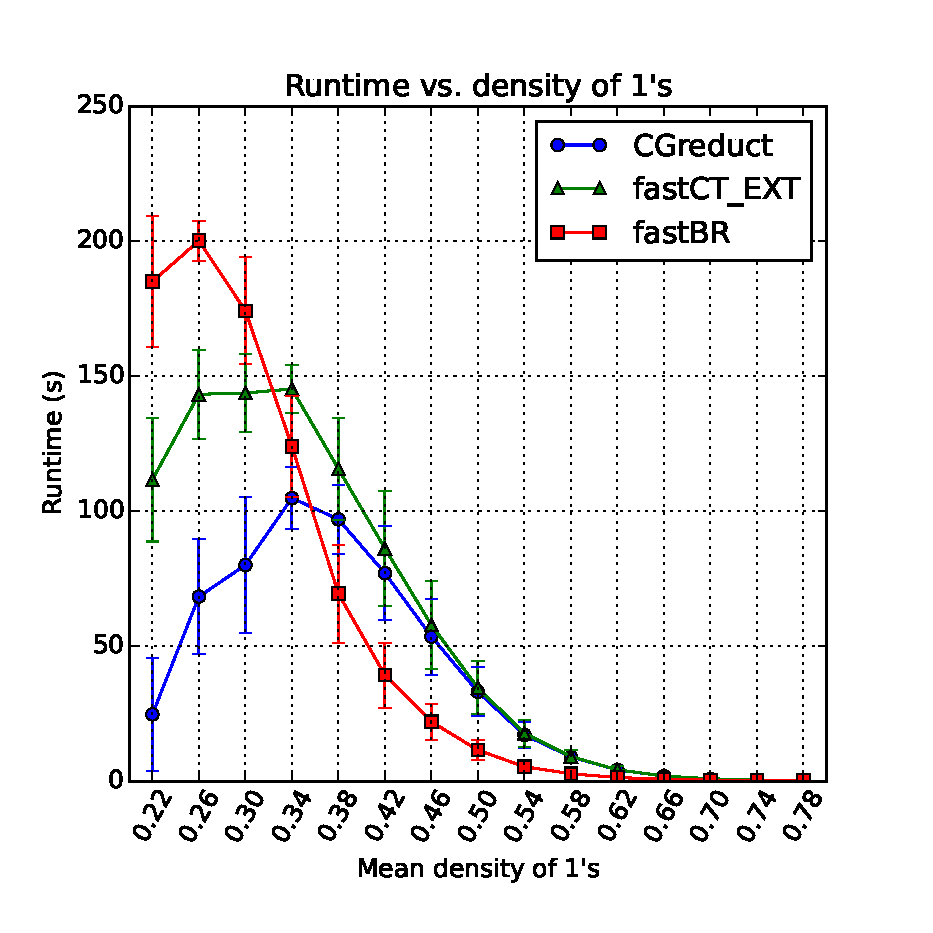
\includegraphics[height=8cm]{overal.eps}
		\end{center}
		\caption{Average algorithms' runtime vs. density of 1's for all synthetic \textit{SBDMs}.}
		\label{fig:scattDensity}
	\end{figure}	

	For clarity purposes, the 500 matrices were split into 15 groups by discretizing the range of densities, each group having approximately 33 \textit{SBDMs}. Figure~\ref{fig:scattDensity} shows the average runtime of all  matrices in each group for the three algorithms, as a function of the density of 1's in the synthetic \textit{SBDMs}. In this figure, the vertical bars show the standard deviation of each bin. 
		
	From Figure~\ref{fig:scattDensity}, we can see that for matrices with density under 0.36  the fastest algorithm was GCreduct, fast--BR was the fastest for matrices with density between 0.36 and 0.66, and the three algorithms show similar performance for matrices with density above 0.66. The fact that high density \textit{SBDMs} do not constitute a complex computational task for reduct computation \citep{Rojas12} is clearly visible in Figure~\ref{fig:scattDensity}. For this reason, a detailed analysis in this region lacks of relevance.
		
	In order to explain the line delimiting those \textit{SBDMs} for which GCreduct is faster than fast--BR (densities under 0.36), we must go deeply into the main difference between these algorithms. The evaluation of the attribute exclusion is the part with the highest complexity within these algorithms ($\Theta (nm)$). This operation is executed more frequently in fast--BR than in GCreduct. The attribute exclusion occurs when there is at least one column in the sub-matrix of the \textit{SBDM}, considering only the attributes in the current candidate, that can be removed without increasing the number of zero rows in this sub-matrix. The exclusion is more frequent in matrices with a higher density of 1's, since it is given by cumulative OR operations. The higher cost of candidate evaluation in fast--BR pays off for \textit{SBDMs} with higher densities (the limit identified from our experiment is 0.36), because supersets of candidates with attribute exclusion are excluded from subsequent evaluations. Take for instance the extreme case of the identity matrix, where there is no exclusion at all, since every attribute is indispensable to form a reduct. For this kind of \textit{SBDMs}, GCreduct needs evaluating as many candidates as fast--BR but the former makes a single verification for exclusion with the set of all attributes. On the other hand, fast--BR verifies the exclusion for each candidate, which leads to a higher computational cost.
	
	Friedman and post hoc Nemenyi-Damico-Wolfe-Dunn tests show that GCreduct was significantly faster (\textit{p--value} $< 10^{-16}$) than fast--CT\_EXT for low (under 0.36) and medium (between 0.36 and 0.66) density matrices. In relation to fast--BR, GCreduct showed a significant runtime reduction (\textit{p--value} $< 10^{-16}$) for low density matrices while it was significantly slower (\textit{p--value} $< 10^{-16}$) for medium density matrices. From this analysis, we conclude that GCreduct is the best algorithm for low density matrices; while fast--BR is the best for medium density matrices. For high (over 0.66) density matrices any algorithm can be used since, as we already commented, computing reducts on this kind of matrices does not constitute a complex computational task. Moreover, from these conclusions, a great advantage can be taken of selecting the appropriate algorithm for each information system. Furthermore, the density of 1's can be computed a priori with a relative low computational cost.
		
	\begin{table}[htb]
		\centering
		\caption{Fast--CText, GCreduct and Fast--BR runtime for information systems from UCI. Sorted by \textit{SBDM} density.}
		\label{tab:density}
		\begin{tabular}{|l|c|r|r|r|}
			\hline
			\multicolumn{1}{|c|}{Information}  && Fast--CText & \multicolumn{1}{c|}{Gcreduct} & \multicolumn{1}{c|}{Fast--BR}  \\
			\multicolumn{1}{|c|}{system}       & Density & runtime (s) & runtime (s)  & runtime (s)  \\
			\hline
			Chess (kr-vs-kp)          & 0.03    & 7.45          & \textbf{$<$0.01} & 0.02            \\
			Keyword-activity          & 0.04    & 1.22          & \textbf{0.42}    & 0.90            \\
			Connect-4                 & 0.05    & 12876.67      & \textbf{44.23}   & 160.61          \\
			QSAR-biodeg               & 0.12    & 0.75          & \textbf{0.19}    & 0.33            \\
			Landsat (train)           & 0.33    & 23797.99      & \textbf{9949.31} & 17732.49        \\
			Dermatology               & 0.34    & 16.02         & 12.25            & \textbf{4.62}   \\
			Credit-g                  & 0.35    & \textbf{0.05} & 0.06             & 0.12            \\
			Flags                     & 0.35    & 1.00          & \textbf{0.74}    & 1.06            \\
			Diabetes                  & 0.38    & 86.99         & \textbf{19.48}   & 23.37           \\
			Student-por               & 0.41    & 1874.57       & 1657.90          & \textbf{161.35} \\
			Sponge                    & 0.42    & 0.63          & 0.58             & \textbf{0.14}   \\
			Student-mat               & 0.43    & 1003.87       & 929.46           & \textbf{81.82}  \\
			Lung-cancer               & 0.47    & 188.20        & 133.43           & \textbf{7.34}   \\
			Waveform                  & 0.50    & 2.11          & 1.88             & \textbf{1.64}   \\
			Cylinder-bands            & 0.55    & 5.03          & 4.59             & \textbf{0.53}   \\
			\hline
		\end{tabular}
	\end{table}
	
	\phantomsection\label{par:kind}
	In Table~\ref{tab:density}, we included the density of 1's and the runtime shown for each \textit{SBDM} in Table~\ref{tab:java}. We also sorted the information systems in Table~\ref{tab:density} in ascending order of the density of 1's in their associated \textit{SBDM}. Although this is a small heterogeneous sample, the rule obtained from synthetic data can be verified in this table. For information systems with \textit{SBDM} densities close to the boundary of 0.36 we cannot conclude which one is the fastest algorithm, as it can be seen in Table~\ref{tab:density}. However, for those information systems which have a \textit{SBDM} with density clearly under 0.36, GCreduct was the fastest. In the same way, fast-BR performed faster for those information systems having a \textit{SBDM} with density clearly above 0.36.
	
	The density of 1's of the \textit{SBDM} is not the only parameter affecting the relative performance of these algorithms. This fact can be verified in Figure~\ref{fig:scattDensity}, where the vertical bars show the standard deviation of the runtime for different \textit{SBDMs} which have the same density. Thus, we may infer that the distribution of 1's within the \textit{SBDM} also has a significant influence, which deserves a deeper study. However, for density values not too close to 0.36 this variations in the distribution of 1's	within the \textit{SBDM} have not effect on the determination of the fastest algorithm, as it can be also seen in Figure~\ref{fig:scattDensity}.\phantomsection\label{par:distribution}

\section{Conclusions}\label{conclusions}
	In this work, we presented a new algorithm, GCreduct, for computing all reducts of an information system. In our proposed algorithm, the search space is traversed evaluating some candidate subsets and, based on pruning properties, many others are discarded. Algorithms reported in the literature use operations with a high cost for candidate evaluation in order to reduce the number of evaluated candidates. The main contribution of our proposal, unlike previous algorithms, is the use of simpler operations for candidate evaluation, based on the pruning properties of gap elimination and attribute contribution, which allows a faster reduct computation. 
	
	After conducting a series of experiments over synthetic \textit{SBDMs} and information systems from the UCI repository, we can conclude that GCreduct performs faster than the fastest previously reported algorithms on those information systems for which their associated \textit{SBDM} has a density of 1's under 0.36. This result provides an instrument to select the proper algorithm for a determined information system. Further studies should be devoted to deeper explore the relation found between the fastest algorithm for reduct computation of an information system, and the density of 1's. 
	
	Finally, since the density of 1's of the \textit{SBDM} is not the only factor that affects the performance of the algorithms, including other factors deserves a wider study as future work. These study should shed light on the influence of the distribution of 1's inside the \textit{SBDM} over the algorithm's performance. 

\section{Acknowledgements}
	The first author gratefully acknowledge CONACyT for his doctoral fellowship, through the scholarship 399547.
%-------------------------------------------------------------------------------
% Bibliography
%-------------------------------------------------------------------------------
\newpage 
\bibliography{mybib}{}
\bibliographystyle{authordate1}
\end{document}
